
\baselineskip=8mm
\chapter{เอกสารและงานวิจัยที่เกี่ยวข้อง}

% \renewcommand{\thesubsection}{\thechapter.\arabic{subsection}}
\numberwithin{equation}{chapter}
\numberwithin{equation}{section}
\renewcommand{\thesubsection}{\arabic{subsection}.}
\renewcommand{\theequation}{\thesection.\arabic{equation}}
\renewcommand{\thesection}{}
\renewcommand{\thesubsubsection}{\thesubsection\arabic{subsubsection}.}



ในการศึกษา ภาคนิพนธ์เรื่อง “แอปพลิเคชันจัดตารางเวรพยาบาล” ผู้จัดทำได้ศึกษาหลักการ ทฤษฎี และงานวิจัยที่เกี่ยวข้อง เพื่อเป็นแนวทางในการศึกษาและพัฒนาภาคนิพนธ์ รายละเอียดหัวข้อดังต่อไปนี้

\hspace{0cm}\subsection{แนวทางการจัดตารางเวรและการเบิกเงินค่าตอบแทนนอกเวลาของพยาบาล}

\hspace{0cm}\subsection{ทฤษฎีการวิเคราะห์และออกแบบระบบ SDLC}

\hspace{0cm}\subsection{ภาษาและเครื่องมือที่ใช้ในการพัฒนา}

\hspace{0cm}\subsection{ทฤษฎีเกี่ยวกับความพึงพอใจ}

\hspace{0cm}\subsection{งานวิจัยที่เกี่ยวข้อง}

\clearpage

\renewcommand{\thesubsection}{}

\section{แนวทางการจัดตารางเวรและการเบิกเงินค่าตอบแทนนอกเวลาของพยาบาล}

\vspace{0.25cm}


อ้างถึงบันทึกของกระทรวงสาธารณะสุขที่ สธ 0202.3.7/ว 79 เรื่อง “ข้อบังคับกระทรวงสาธารณะสุขว่าด้วยการจ่ายเงินค่าตอบแทนเจ้าหน้าที่ที่ปฏิบัติงานให้กับหน่วยบริการในสังกัดกระทรวงสาธารณะสุข พ.ศ.2566 หลักเกณฑ์วิธีการและเงื่อนไขการจ่ายเงินค่าตอบแทน จำนวน 5 ฉบับ” ลงไว้เมื่อ 3 กุมภาพันธ์ 2566 ได้มีการปรับปรุงข้อบังคับฯ ดังกล่าว เพื่อให้มีความเหมาะสมกับภาวะเศรษฐกิจในปัจจุบัน และเพื่อให้เกิดความเข้าใจตรงกัน ในเรื่องการเบิกเงินค่าตอบแทนนออกเวลา (Over Time, OT) และค่าเวรหรือพลัดของพยาบาลวิชาชีพ พยาบาลเทคนิค ผู้ช่วยพยาบาล รวมทั้งให้เกิดความถูกต้องและเป็นธรรม ในเรื่องการบริหารจัดการชั่วโมงการทำงานของพยาบาล กระทรวงสาธารณสุข จึงมีหลักการและแนวทางปฎิบัติที่ผู้บริหารและผู้เกี่ยวข้องสามารถนำไปดำเนินการ ดังนี้

\hspace{0pt}\subsection{หลักการ}


\hspace{0.5cm}\hangindent=2.6cm\hangafter=1\subsubsection{เวรเช้า ผลัดบ่าย ผลัดดึก (เวรพลัดๆละ 8 ชั่วโมง) เป็นการปฏิบัติงานตามปกติของพยาบาลวิชาชีพ พยาบาลเทคนิค ผู้ช่วยพยาบาล เนื่องจากเป็นผู้ที่ปฏิบัติงานผลัดเปลี่ยนหมุนเวียนกันดูแลผู้ป่วยตลอด 24 ชั่วโมง}

\hspace{0.5cm}\hangindent=2.6cm\hangafter=1\subsubsection{การปฏิบัติงานของพยาบาลวิชาชีพ พยาบาลเทคนิค ผู้ช่วยพยาบาล แต่ละเดือนจะมีจำนวนเวรเท่ากับวันทำการในของเดือนนั้นๆ นับว่าเป็นการปฏิบัติงานโดยปกติของพยาบาล นอกเหนือจากจำนวนเวรดังกล่าวจึงเป็นการปฏิบัติงานนอกเวลา (Over Time, OT)}

\hspace{0.5cm}\hangindent=2.6cm\hangafter=1\subsubsection{ในแต่ละเวรหรือผลัด ควรกำหนดให้มีพยาบาลวิชาชีพที่มีศักยภาพการปฏิบัติงานต่างระดับอย่างน้อย 2 ระดับ (Skill mix) ขึ้นไป}

\hspace{0.5cm}\hangindent=2.6cm\hangafter=1\subsubsection{การเบิกงานค่าตอบแทนนอกเวลา (Over Time, OT) เบิกจากจำนวนเวรหรือผลัดที่เกินจากการจัดเวรหรือผลัดปกติ โดยสามารถเบิกได้ทั้งเวรเช้า หรือผลัดบ่าย หรือผลัดดึก}

\hspace{0.5cm}\hangindent=2.6cm\hangafter=1\subsubsection{การเบิกเงินค่าผลัดบ่าย หรือผลัดดึก มีจัดให้เป็นการเบิกเงินในการปฏิบัติงานปกติไม่ใช่การปฏิบัติงานนอกเวลา (Over Time, OT)}

\hspace{0.5cm}\hangindent=2.6cm\hangafter=1\subsubsection{เวรเช้า ผลัดบ่าย ผลัดดึก สามารถจัดเวรเสริมได้ตามภาระงานที่กำหนด และเวรเสริมนั้นจะเบิกเงินค่าตอบแทนนอกเวลา (Over Time, OT)}

\clearpage

\hspace{0pt}\subsection{นโยบายกลุ่มการพยาบาล}

\hspace{0.5cm}\hangindent=2.6cm\hangafter=1\subsubsection{ให้จัดทำตารางรูปแบบการจัดเวรแบบล็อคเวรผลัด เช่น ช/ช/ด/ด/บ/บ หรือ ช/ช/ด/ด/ด/บ หรือ ช/ช/ช/ด/บ/บ หรืออย่างอื่นเป็นต้น (เฉลี่ยเวรเข้า ผลัดบ่าย และผลัดดึก ให้พยาบาลแต่ละคนในหน่วยงานเท่าๆกัน)}

\hspace{0.5cm}\hangindent=2.6cm\hangafter=1\subsubsection{การแลกเวร/เปลี่ยนเวร จะสามารถแลกเปลี่ยนเวรได้ในพยาบาลที่มีศักยภาพการปฏิบัติงานในระดับเดียวกัน โดยได้รับอนุญาต และแก้ไขตารางเวรจากหัวหน้าหน่วยงานหรือผู้ที่ได้รับมอบหมายเท่านั้น}

\hspace{0.5cm}\hangindent=2.6cm\hangafter=1\subsubsection{การกำหนดเพิ่มและลดจำนวนพยาบาลที่ปฏิบัติงาน พิจารณาจากภาระงานซึ่งประกอบด้วยจำนวนผู้ป่วยและประเภทของผู้ป่วย}

\hspace{0.5cm}\hangindent=2.6cm\hangafter=1\subsubsection{หัวหน้าหน่วยงานตรวจสอบจำนวนชั่วโมงการทำงานต่อสัปดาห์ของพยาบาล โดยหลีกเลี่ยงการปฏิบัติงานากกว่า 60 ชั่วโมงต่อสัปดาห์ หรือมากกว่า 12 ชั่วโมงต่อเวรติดกันเกิน 3 วัน}

\hspace{0.5cm}\hangindent=2.6cm\hangafter=1\subsubsection{ต้องให้หัวหน้าหน่วยงานตรวจสอบและเซ็นรับรองตารางเวรแต่ละเดือน หลังจากพิจารณาว่าเป็นไปตามแนวทางการปฏิบัติข้อ 1-4}

\vspace{0.5cm}

\hspace{0pt}\subsection{แนวทางปฏิบัติ}

\hspace{0.5cm}\hangindent=2.6cm\hangafter=1\subsubsection{การเฉลี่ยวันหยุดที่ตรงกับวันเสาร์ วันอาทิตย์และวันนักขัตฤกษ์ ควรจัดจำนวนเวรให้กระจายอย่างเหมาะสมกับพยาบาลวิชาชีพ พยาบาลเทคนิค ผู้ช่วยพยาบาล}

\hspace{0.5cm}\hangindent=2.6cm\hangafter=1\subsubsection{การจัดเวรหรือผลัด และการจัดเวรหรือผลัดที่เป็นการปฏิบัติงานนอกเวลาควรเฉลี่ยจำนวนเวรหรือผลัดให้มีความเหมาะสมกันของพยาบาลในระดับเดียวกัน}

\hspace{0.5cm}\hangindent=2.6cm\hangafter=1\subsubsection{การกำหนดหน้าที่รับผิดชอบของพยาบาลวิชาชีพ พยาบาลเทคนิค ผู้ช่วยพยาบาลแต่ละคนในแต่ละเวรผลัดเพื่อให้เกิดการทำงานเป็นทีมที่มีประสิทธิภาพในการดูแลผู้ป่วย}

\hspace{0.5cm}\hangindent=2.6cm\hangafter=1\subsubsection{หัวหน้าหน่วยงาน ตรวจสอบ จำนวนชั่วโมงการทำงานต่อสัปดาห์ของพยาบาล โดยหลีกเลี่ยงการปฏิบัติงานากกว่า 60 ชั่วโมงต่อสัปดาห์ หรือมากกว่า 12 ชั่วโมงต่อเวรติดกันเกิน 3 วัน}

\hspace{0.5cm}\hangindent=2.6cm\hangafter=1\subsubsection{หัวหน้าหน่วยงานตรวจสอบและเซ็นรับรองตารางเวรแต่ละเดือน หลังจากพิจารณาว่าเป็นไปตามแนวทางการปฏิบัติข้อ 1-4}


\clearpage


\section{ทฤษฎีการวิเคราะห์และออกแบบระบบ SDLC}

\begin{figure}[h!]
    \centering
    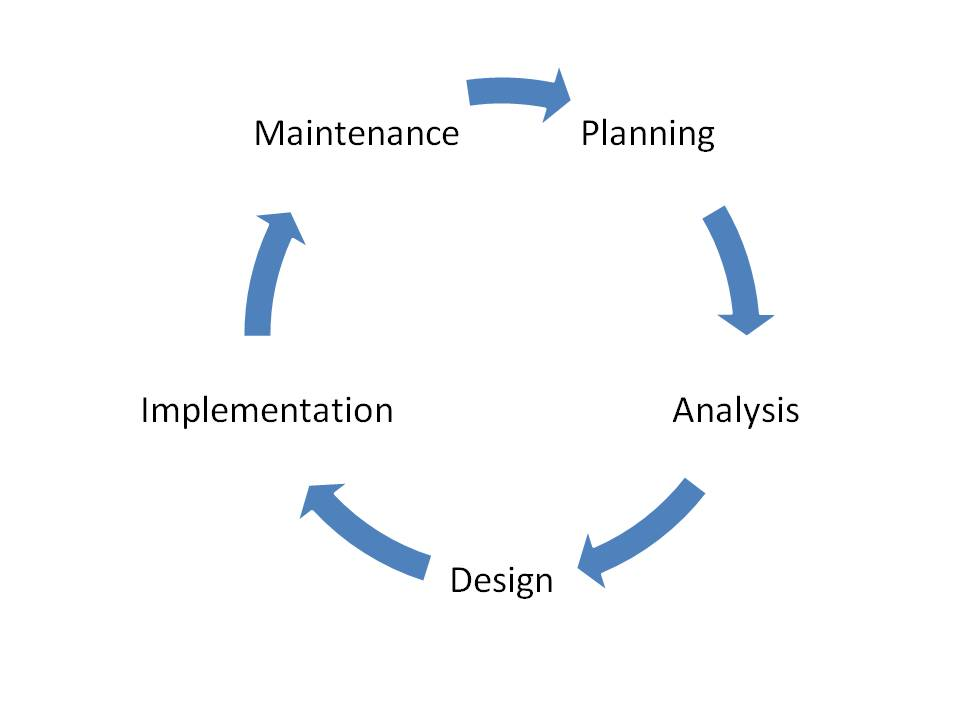
\includegraphics[width=0.6\textwidth]{SDLC.jpeg}
    \caption{ภาพแสดงขั้นตอนของระบบวงจรชีวิตการพัฒนาระบบ (SDLC)}
\end{figure}

\vspace{-1cm}

\begin{center}\textbf{ที่มา:} Gary Newport, 2013\end{center}
\vspace{0.5cm}

ปกติแล้วคำว่า วงจรชีวิต (Life Cycle) มักจะใช้กับสิ่งมีชีวิตบนพื้นโลก ไม่ว่าจะเป็นวงจรชีวิตของมนุษย์ สัตว์ หรือพืช ซึ่งข้องเกี่ยวกับการเกิด การดำเนินชีวิต และการตาย ในทำนองเดียวกัน เมื่อนำวงจรชีวิตนี้มาใช้กับซอฟต์แวร์ ก็จะเป็นการอธิบายถึงขั้นตอนการพัฒนาซอฟต์แวร์ ซึ่งเรียกว่า วงจรชีวิตการพัฒนาซอฟต์แวร์ (Software Development Life Cycle, SDLC) ซึ่งเป็นขั้นตอนการพัฒนาซอฟต์แวร์ที่มีการจัดเป็นขั้นตอนตามลำดับ และมีการทำงานร่วมกันของทีมงานที่เกี่ยวข้อง โดยมีขั้นตอนหลักๆ ดังนี้ \cite{sdlc}

\subsubsection{การวางแผนโครงการ (Project Planning Phase)}

\subsubsection{การวิเคราะห์ (Analysis Phase)}

\subsubsection{การออกแบบ (Design Phase)}

\subsubsection{การนำไปใช้ (Implementation Phase)}

\subsubsection{การบำรุงรักษา (Maintenance Phase)}


\clearpage

\section{ภาษาและเครื่องมือที่ใช้ในการพัฒนา}

\vspace{0.25cm}

\hspace{0cm}\subsection{การพัฒนาระบบจัดตารางเวรพยาบาลมีการนำเอาเทคโนโลยีหลากหลายด้านเข้ามาใช้ในการพัฒนา โดยการพัฒนาจะมีการแบ่งเป็น 2 ส่วนหลักๆ คือ ส่วนของหน้าบ้าน (Frontend) และส่วของหลังบ้าน (Backend) และมีการใช้เทคโดนโลยีเกี่ยวกับฐานข้อมูล คลาวด์ และอื่นๆดังนี้}

\hspace{0cm}\subsubsection{ภาษาที่ใช้ในการพัฒนาส่วนของหน้าบ้าน คือ ภาษา JavaScript ซึ่งเป็นภาษาที่ใช้ในการพัฒนาเว็บแอปพลิเคชัน และเป็นภาษาที่ใช้ในการพัฒนาเว็บเซอร์วิส โดยใช้ Framework ที่ชื่อว่า React ซึ่งเป็น JavaScript library ที่ใช้สำหรับสร้าง user interface ที่ให้เราสามารถเขียนโค้ดในการสร้าง UI ที่มีความซับซ้อนแบ่งเป็นส่วนเล็กๆออกจากกันได้ ซึ่งแต่ละส่วนสามารถแยกการทำงานออกจากกันได้อย่างอิสระ และทำให้สามารถนำชิ้นส่วน UI เหล่านั้นไปใช้ซ้ำได้อีก} \cite{React}

\hspace{0cm}\subsubsection{ภาษาที่ใช้ในการพัฒนาส่วนของหลังบ้าน คือ ภาษา Go ซึ่งเป็นภาษาที่เป็นโอเพ่นซอร์ส (OpenSource) ที่พัฒนาโดยบริษัทกูเกิ้ล (Google) \cite{Go} โดยใช้ Gin ซึ่งถูกพัฒนาต่อมาจาก Martini ที่หยุดพัฒนาไปแล้ว โดย Gin จะใช้ customized httprouter ทำให้มีประสิทธิภาพด้านความเร็วที่สูงมาก เป็น framework ที่มี performance กับ productivity ที่ดี \cite{Gin} และมีการใช้ Gorm ซึ่งเป็น Library ของ ORM สำหรับใช้งานในภาษา Golang ที่ช่วยให้เราสามารถแมปข้อมูลระหว่าง Relational Database กับภาษาโปรแกรมมิ่งที่เขียนแบบ OOP โดยจะทำให้เราไม่จำเป็นต้องเขียนคำสั่ง SQL เอง แต่จะเป็นการเขียนในรูปแบบคำสั่งของภาษาโปรแกรมมิ่งนั้น ๆ ได้เลย ทำให้ลดความซับซ้อนของการติดต่อหรือมี Interact กับฐานข้อมูล \cite{Gorm}} 

\hspace{0cm}\subsubsection{มีการใช้ Mysql ซึ่งเป็นระบบจัดการฐานข้อมูล หรือ Database Management System (DBMS) แบบข้อมูลเชิงสัมพันธ์ หรือ Relational Database Management System (RDBMS) ซึ่งเป็นระบบฐานข้อมูลที่จัดเก็บรวบรวมข้อมูลในรูปแบบตาราง โดยมีการแบ่งข้อมูลออกเป็นแถว (Row) และในแต่ละแถวแบ่งออกเป็นคอลัมน์ (Column) เพื่อเชื่อมโยงระหว่างข้อมูลในตารางกับข้อมูลในคอลัมน์ที่กำหนด แทนการเก็บข้อมูลที่แยกออกจากกัน โดยไม่มีความเชื่อมโยงกัน ซึ่งประกอบด้วยข้อมูล (Attribute) ที่มีความสัมพันธ์เชื่อมโยงกัน (Relation) โดยใช้ RDBMS Tools สำหรับการควบคุมและจัดเก็บฐานข้อมูลที่จำเป็น ทำให้นำไปประยุกต์ใช้งานได้ง่าย ช่วยเพิ่มประสิทธิภาพในการทำงานให้มีความยืดหยุ่นและรวดเร็วได้มากยิ่งขึ้น รวมถึงเชื่อมโยงข้อมูล ที่จัดแบ่งกลุ่มข้อมูลแต่ละประเภทได้ตามต้องการ จึงทำให้ MySQL เป็นโปรแกรมระบบจัดฐานข้อมูลที่ได้รับความนิยมสูง \cite{sql}}

\clearpage

\hspace{0cm}\subsubsection{ในการเขียนโปรแกรมจะมีตัวช่วยคือ Code Editor โดยในการพัฒนาจะใช้ Visual Studio Code หรือ VSCode เป็นโปรแกรม Code Editor ที่ใช้ในการแก้ไขและปรับแต่งโค้ด จากค่ายไมโครซอฟท์ มีการพัฒนาออกมาในรูปแบบของ OpenSource จึงสามารถนำมาใช้งานได้แบบฟรี ๆ ที่ต้องการความเป็นมืออาชีพ ซึ่ง Visual Studio Code นั้น เหมาะสำหรับนักพัฒนาโปรแกรมที่ต้องการใช้งานข้ามแพลตฟอร์ม รองรับการใช้งานทั้งบน Windows, macOS และ Linux สนับสนุนทั้งภาษา JavaScript, TypeScript และ Node.js สามารถเชื่อมต่อกับ Git ได้ นำมาใช้งานได้ง่ายไม่ซับซ้อน มีเครื่องมือส่วนขยายต่าง ๆ ให้เลือกใช้อย่างมากมาก \cite{vscode}}

\hspace{0cm}\subsubsection{มีการใช้ Container ในการพัฒนา โดยใช้ Docker เป็นแพลตฟอร์มซอฟต์แวร์ที่ช่วยให้สร้าง ทดสอบ และติดตั้งแอปพลิเคชันใช้จริงได้อย่างรวดเร็ว Docker จะบรรจุซอฟต์แวร์ลงไปในหน่วยที่เป็นมาตรฐานเรียกว่า คอนเทนเนอร์ ซึ่งจะมีทุกสิ่งที่ซอฟต์แวร์ต้องใช้ในการเรียกใช้งาน รวมทั้งไลบรารี เครื่องมือสำหรับระบบ โค้ด และรันไทม์ เมื่อใช้ Docker จะสามารถติดตั้งใช้จริงและปรับขนาดแอปพลิเคชันให้เหมาะกับทุกสภาพแวดล้อมและทราบว่าโค้ดจะเรียกใช้ได้อย่างอย่างรวดเร็ว \cite{docker} และมีการจัดการคอนเทนเนอร์ด้วย Kubernetes ซึ่งเป็น container orchestration engine. จุดประสงค์หลักของ kubernetes คือการจัดการ container deployments. ในปัจจุบันทุกๆ application กำลังจะใช้ Microservices architecture มากกว่า Monolithic architecture. และ วิธีการใช้งาน microservices architecture เหล่านั้นจะออกแบบโดย containerization technology. ตามที่เรารู้ Docker ปฏิวัติ container technology. ทุกคนใช้ containers ในการ build their applications ในตอนนี้และวิธีการ manage containers at a large scale, kubernetes ถูกออกแบบและพัฒนาโดย Google และปัจจุบัน Project ถูกดูแลโดย Cloud Native Computing Foundation.\cite{kubernetes}}

\hspace{0cm}\subsubsection{ในการใช้งาน Software Development Life Cycle (SDLC) จะใช้ Git ซึ่งเป็นระบบควบคุมเวอร์ชัน (Version Control System) ที่ถูกออกแบบมาเพื่อใช้ในการจัดการโค้ดของโปรเจค โดย Git จะช่วยให้นักพัฒนาสามารถทำงานร่วมกันได้ โดยที่ไม่ต้องกังวลเรื่องการทับซ้อนกัน และสามารถทำงานได้ทั้งออนไลน์และออฟไลน์ และสามารถอัปโหลดโปรแกรมในแต่ละเวอร์ชันได้ \cite{git}}

\hspace{0cm}\subsubsection{มีการใช้งานเกี่ยวกับ Cloud ซึ่งเป็นเครื่องมือหรือ การบริการ System Host (ระบบที่เป็นตัวกลางไว้ควบคุม System อื่นๆ) ต่างๆผ่านอินเทอร์เน็ต \cite{cloud} โดยจะใช้ AWS ซึ่งเป็นแพลตฟอร์มด้าน “Cloud Computing“ ที่มีส่วนแบ่ง Market Share ในตลาดคลาวด์มากที่สุดในโลก อ้างอิงจาก Synergy Research Group โดย AWS ย่อมาจาก Amazon Web Services เป็นบริษัทลูกของ Amazon ให้บริการเช่าเครื่องมือต่าง ๆ ที่ประมวลผลบนระบบคลาวด์ มีให้เลือกใช้งานหลากหลายและครบครันทุกโซลูชันสำหรับองค์กรในยุคดิจิทัล ไม่ว่าจะเป็น Server, Networking, Database, Application Services \cite{aws}}


\section{ทฤษฎีเกี่ยวกับความพึงพอใจ}

\hspace{0cm}\subsection{ในการประเมินความพึงพอใจของผู้ใช้งานระบบที่สร้างขึ้นให้ครอบคลุมวัตถุประสงค์ ในการประเมินความพึงพอใจจะเป็นการประเมินแบบ มาตราส่วนประเมินค่า (Rating Scale) 5 ระดับโดยใช้แบบสอบถาม โดยแบบสอบถามจะเป็นข้อความเชิงบวกทั้งหมดโดยแบ่งออกเป็น 4 ด้าน ได้แก่ ด้านความถูกต้องในการใช้งานระบบ ด้านความสะดวกและความง่ายในการใช้งานระบบ ด้านความปลอดภัยและความเป็นส่วนตัวของข้อมูล ด้านความสวยงามของระบบ โดยจะนำข้อมูลจากแบบสอบถามมาแปรผลโดยใช้ค่าเฉลี่ย}

\vspace{0.25cm}

\begin{table}[h]
    \captionsetup{justification=raggedright,singlelinecheck=false}
    \centering
    \fontsize{12}{20}\selectfont	
    \begin{tabular}{c l}
            \hline
            คะแนนเฉลี่ย  & ระดับความพึงพอใจ \\
            \hline
            4.50 - 5.00 & พึงพอใจมากที่สุด \\
            3.50 - 4.49 & พึงพอใจมาก \\
            2.50 - 3.49 & พึงพอใจปานกลาง \\
            1.50 - 2.49 & พึงพอใจน้อย \\
            1.00 - 1.49 & พึงพอใจน้อยที่สุด\\
            \hline
        \end{tabular}
    \caption{หลักการแปรค่าเฉลี่ยความพึงพอใจของผู้ใช้งานระบบ}
\end{table}

\renewcommand{\thesubsection}{\arabic{subsection}.}

\section{งานวิจัยที่เกี่ยวข้อง}

\vspace{0.25cm}


\hspace{0cm}\subsection{ต้นทุุนและผลผลิตทางการพยาบาลระหว่างวีธีจัดตารางเวรแบบปกติกับแบบใหม่ของฝ่ายการพยาบาลโรงพยาบาลเอกชนแห่งหนึ่ง การวิจัยกึ่งทดลองนี้มีวัตถุประสงค์เพื่อเปรียบเทียบต้นทุนและผลผลิตทางการพยาบาลระหว่างการจัดตารางเวรแบบปกติกับแบบใหม่ของฝ่ายการพยาบาลโรงพยาบาลเอกชนขนาด 120 เตียง กลุ่มตัวอย่าง คือ รายงานต้นทุนค่าปฏิบัติ งานนอกเวลาและผลผลิตทางการพยาบาลที่มาจากการปฏิบัติงานของบุคคลากรทางการพยาบาลของฝ่ายผู้ป่วยนอก จำนวนทั้งหมด 84 คน เครื่องมือที่ใช้ในการวิจัย ประกอบด้วยแนวทางการจัดตารางเวรแบบใหม่ คู่มือการจัดตารางเวรแบบใหม่ แบบบันทึกข้อมูลต้นทุน และแบบบันทึกผลผลิตทางการพยาบาลของฝ่ายการพยาบาล วิเคราะห์ข้อมูลด้วยสถิติ เชิงพรรณนาและทดสอบค่าที  ผลการวิจัยพบว่า ค่าเฉลี่ยต้นทุนค่าปฏิบัติงานนอกเวลาโดยรวมของฝ่ายผู้ป่วยนอกด้วยการจัดตารางเวรปกติเท่ากับ 170,646.00 บาท และการจัดตารางเวรใหม่เท่ากับ 137,899.20บาท พบว่า ค่าเฉลี่ยต้นทุนค่าปฏิบัติงานนอกเวลาโดยรวมระหว่างการจัดตารางเวรแบบปกติและการจัดตารางเวรแบบใหม่มีความแตกต่างกันอย่างมีนัยสำคัญ ทางสถิติ (p < .05) และค่าเฉลี่ยผลผลิตทางการพยาบาลโดยรวมของฝ่ายผู้ป่วยนอกระหว่างการจัดตารางเวรแบบปกติ และแบบใหม่มีความแตกต่างกันอย่างมีนัยสำคัญทางสถิติ (p < .05) โดยการจัดตารางเวรแบบใหม่ (ร้อยละ 110.58) ซึ่งใกล้เคียงกับค่ามาตรฐานมากกว่าการจัดตารางเวรแบบปกติ (ร้อยละ 120.80) ผลการวิจัยมีข้อเสนอแนะว่า ผู้บริหารควรมีการออกแบบงานการจัดตารางเวรแบบใหม่เพื่อช่วยทำให้การบริหารต้นทุนมีประสิทธิภาพและเกิดผลิตผลทางการพยาบาลตามเป้าหมาย \cite{vijai1}}

\hspace{0cm}\subsection{การพัฒนาโปรแกรมจัดตารางเวรอัตโนมัติของนักรังสีเทคนิค : กรณีศึกษาแผนกรังสีวินิจฉัย โรงพยาบาลสงขลานครินทร์ โรงพยาบาลสงขลานครินทร์ได้มีการจัดตารางเวรโดยบุคลากรที่เป็นนักรังสีเทคนิคที่มีประสบการณ์หรือเป็นหัวหน้าภายในแผนกโดยการจัดตารางเวรนั้นมีองค์ประกอบในการจัดตารางเวรที่หลากหลายมากทำให้ใช้เวลานานส่งผลให้เสียอัตรากำลังของนักรังสีเทคนิคสำหรับปฏิบัติงานประจำนอกจากนี้อาจเกิดความผิดพลาดและไม่เหมาะสมกับนักรังสีเทคนิคแต่ละคนเพื่อแก้ปัญหาดังกล่าวทางผู้วิจัยได้ออกแบบโปรแกรมอัตโนมัติสำหรับใช้ในการช่วยจัดตารางเวรให้กับแผนกรังสีวินิจฉัยโรงพยาบาลสงขลานครินทร์ วิธีการศึกษา : พัฒนาโปรแกรมโดย Visual Studio Code ที่เขียนด้วยภาษา Python และสร้าง GUI ที่ได้ออกแบบมาจากโปรแกรม Figma จากนั้นประเมินความพึงพอใจของผู้ใช้งานโปรแกรมโดยนักรังสีเทคนิคจำนวน 29 คนที่ประจำการอยู่เวรนอกเวลาราชการสังกัดสาขารังสีวินิจฉัย โรงพยาบาลสงขลานครินทร์โดยประเมินภาพรวมของตารางเวรที่โปรแกรมจัดตารางเวรอัตโนมัติสร้างขึ้นจำนวน 10 ข้อโดยแต่ละข้อมีคะแนนเต็ม 5 ผลการศึกษา:ค่าเฉลี่ยและส่วนเบี่ยงเบนมาตรฐานของคะแนนความพึงพอใจเกี่ยวกับตารางเวรที่จัดไม่มีความผิดพลาดมีความถูกต้องเหมาะสมเท่ากับ 4.59 ± 0.50, ตารางเวรที่จัดสามารถเห็นภาพรวมของเจ้าหน้าที่ทั้งระบบได้ชัดเจนเท่ากับ 4.59 ± 0.68, ตารางเวรที่จัดมีความเหมาะสมเท่ากับ 4.45± 0.74, ตารางเวรที่จัดขึ้นรูปแบบใช้งานที่คุ้นเคยเท่ากับ 4.59 ± 0.50, ความสะดวกในการใช้งานระบบเท่ากับ4.66± 0.48, ตารางเวรสามารถจัดการปัญหาการลาล่วงหน้าในการจัดเวรได้เท่ากับ 4.79 ± 0.41, ความพึงพอใจต่อการท างานของโปรแกรมโดยรวมเท่ากับ 4.41± 0.68, ตารางเวรสามารถจัดการปัญหาการลาล่วงหน้าในการจัดเวรได้เท่ากับ 4.69 ± 0.47, ตารางเวรสามารถจัดการปัญหาการลาล่วงหน้าในการจัดเวรได้เท่ากับ5.00, โปรแกรมมีความทันสมัยตัวอักษรชัดเจนเท่ากับ 4.62 ± 0.49 ตามล าดับสรุปผลการศึกษา:การพัฒนาโปรแกรมจัดตารางเวรอัตโนมัติส่งผลให้การจัดเวรมีประสิทธิภาพลดความผิดพลาดต่างๆทำให้มีความสะดวกมากขึ้นลดระยะเวลาในการจัดตารางเวรเพื่อป้องกันและแก้ไขปัญหาการจัดตารางเวรที่ไม่เป็นธรรมกับบุคลากรภายในแผนกรังสีวินิจฉัยโรงพยาบาลสงขลานครินทร์ \cite{vijai2}}

\hspace{0cm}\subsection{การศึกษาลักษณะครอนอไทป์ และความต้องการรูปแบบการจัดตารางการปฏิบัติงานของพยาบาล โรงพยาบาลสังกัดมหาวิทยาลัย ได้จัดทำเพื่อศึกษาลักษณะครอนอไทป์ และความต้องการรูปแบบการจัด ตารางการปฏิบัติงานของพยาบาล การออกแบบการวิจัยเป็นการวิจัยเชิงพรรณา (descriptive study) ดำเนินการวิจัยโดย กลุ่มตัวอย่างเป็นพยาบาล จำนวน 831 คน ปฏิบัติงานหมุนเวียนแบบผลัด อายุงาน 1 ปีขึ้นไป ปฏิบัติงานเวร บ่าย/ดึก  อย่างน้อย 1 เวรต่อเดือน  สังกัดฝ่ายการพยาบาล โรงพยาบาลสังกัดมหาวิทยาลัย  เก็บรวบรวมข้อมูลจากแบบสอบถามผ่าน Google Form  แบบสอบถามประกอบด้วย 3 ส่วน คือ ข้อมูลส่วนบุคคล  ความต้องการรูปแบบการจัดตารางการปฏิบัติงาน และแบบวัด Morningness - Eveningness Questionnaires ฉบับภาษาไทย (T-MEQ)  วิเคราะห์ข้อมูลโดยใช้จำนวน ร้อยละ และ สถิติทดสอบไคสแควร์ (chi-squared test) ผลการวิจัยพบว่าพยาบาลจำนวน 831 คน  ส่วนใหญ่มีลักษณะครอนอไทป์เป็นอินเทอมิเดียไทป์ (ร้อยละ 64.7) ซึ่งมีความสัมพันธ์กับความต้องการการปฏิบัติงานเหลื่อมเวลาเวรดึก  การปฏิบัติงาน 10 ชั่วโมงต่อวัน การปฏิบัติงานแบบเวรเดียวตลอด   ประสบการณ์ในการทำงานประเภทผู้ป่วยที่ ดูแล  สถานภาพสมรส และภาระที่ต้องรับผิดชอบ อย่างมีนัยสำคัญทางสถิติ (p<0.05) ความต้องการรูปแบบการจัดตารางการปฏิบัติงานส่วนใหญ่พยาบาลมีความต้องการปฏิบัติงาน เวรเช้า (ร้อยละ 51.4)  ปฏิบัติงานเหลื่อมเวลาเวรเช้า (ร้อยละ 73.9) และต้องการเลือกวันหยุดได้ด้วยตนเอง (ร้อยละ 93.5)  พยาบาลส่วนใหญ่ไม่ต้องการหมุนเวียนหน่วยงาน (ร้อยละ 90.5) และไม่เลือกปฏิบัติงานแบบเวรเดียวตลอด (ร้อยละ 65.8) ประสบการณ์ในการทำงาน ประเภทผู้ป่วยที่ดูแล สถานภาพสมรสและภาระที่ต้องรับผิดชอบ มีความสัมพันธ์กับความต้องการรูปแบบการจัดตารางการปฏิบัติงานในการขึ้นเวรผลัด และการปฏิบัติงาน แบบเวรเดียวตลอด  อย่างมีนัยสำคัญทางสถิติ (p<0.05)โดยมีข้อเสนอแนะคือ ผู้บริหารองค์กรควรสอบถามลักษณะครอนอไทป์ ความต้องการรูปแบบการจัดตารางการปฏิบัติงานและเปิดโอกาสให้พยาบาลได้เลือกเวรที่ต้องการและปรับรูปแบบการจัดเวรให้มีความยืดหยุ่น \cite{vijai3}}

\hspace{0cm}\subsection{การจัดตารางงานของสัตวแพทย์ในโรงพยาบาลสัตว์ด้วยวิธีแบบจําลองกําหนดการเชิงจํานวนเต็ม : กรณีศึกษา โรงพยาบาลสัตว์แห่งหนึ่งในจังหวัดนครปฐม โรงพยาบาลสัตว์เป็นสถานที่สําหรับรักษาสัตว์เลี้ยงซึ่งดําเนินการรักษาโดยสัตวแพทย์โดยทั่วไปโรงพยาบาลสัตว์จะมีสัตวแพทย์ประจําอยู่หลายคนทางโรงพยาบาลจะต้องมีการจัดตารางการทํางานของสัตว์แพทย์ว่าสัตวแพทย์แต่ละคนจะต้องปฏิบัติงานในช่วงเวลาใดการจัดตารางงานที่เหมาะสมให้กับสัตวแพทย์มีความสําคัญอย่างยิ่งเพราะตารางงานที่เหมาะสมจะช่วยให้สัตวแพทย์ทําการรักษาสัตว์ได้อย่างมีประสิทธิภาพมากยิ่งขึ้นงานวิจัยนี้ได้นําเสนอแบบจําลองกําหนดการเชิงจํานวนเต็มสําหรับจัดตารางงานของสัตวแพทย์ใน 1 สัปดาห์โดยใช้ข้อมูลจากโรงพยาบาลสัตว์แห่งหนึ่งในจังหวัดนครปฐมวัตถุประสงค์ของแบบจําลองที่นําเสนอคือต้องการให้ผลรวมของจํานวนวันหยุดของสัตวแพทย์ทั้งหมดมีค่ามากที่สุดแบบจําลองที่นําเสนอนี้จะให้ผลเฉลยเป็นตารางการปฏิบัติงานของสัตวแพทย์ทั้งหมดใน 1 สัปดาห์ซึ่งให้ข้อมูลว่าสัตวแพทย์คนใดต้องเข้าปฏิบัติงานในช่วงเวลาใดในงานวิจัยนี้แบบจําลองที่นําเสนอถูกแก้ด้วยโปรแกรมILOG OPL CPLEX 12.6 ผลการทดลองพบว่าจากข้อมูลของโรงพยาบาลกรณีศึกษาซึ่งมีจํานวนสัตวแพทย์ทั้งหมด9 คนเมื่อจัดตารางงานโดยใช้แบบจําลองที่นําเสนอจะได้ผลรวมของจํานวนวันหยุดที่มากที่สุดภายใต้เงื่อนไขการปฏิบัติงานที่โรงพยาบาลกําหนดคือ 28 วันโดยใน 1 สัปดาห์สัตวแพทย์แต่ละคนจะมีวันปฏิบัติงาน 3 ถึง 4 วันแบบจําลองที่นําเสนอนี้สามารถใช้เป็นทางเลือกในการหาตารางการทํางานที่เหมาะสมของสัตวแพทย์ในโรงพยาบาลกรณีศึกษาหรือสามารถนําไปประยุกต์ใช้ได้ \cite{vijai4}}

